
\begin{document}

This section covers the design choices associated with the actively loaded differential amplifier with cascoded current mirror and a class B amplifier for an output stage. Frequency compensation will also be considered in the development to ensure stability.

The circuit that was developed in task 4 will be used for the purposes of this circuit development section. The output stage will be added in this task which will be a class B amplifier. The class B amplifier will consist of a 2n3904 NPN BJT and a 2n3906 PNP BJT. The simulations were conducted in Microcap 10. As these schematics are difficult to read, a set of schematics with identical values and components were created in Eagle by Autodesk. The simulated schematic can be seen in Figure \ref{fig:simschem} below.

\begin{figure}[H]
	\centering
	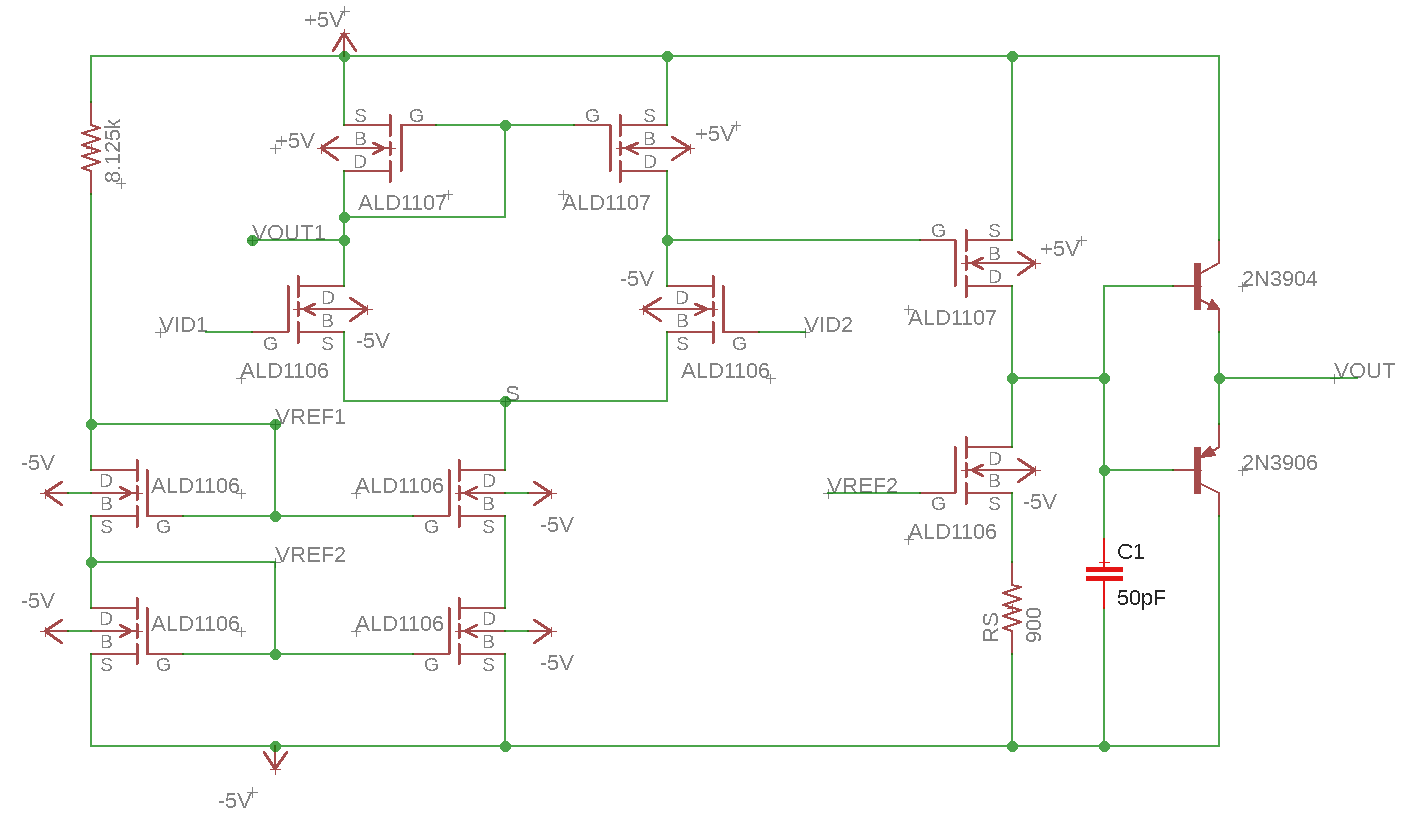
\includegraphics[width=0.8\linewidth]{CircuitDevelopment/schematicsimulation.png}
	\caption{Simulated Circuit}
	\label{fig:simschem}
\end{figure}



\end{document}